\documentclass[letterpaper]{article}
\usepackage[submission]{aaai2027}
\usepackage[hyphens]{url}
\usepackage{graphicx}
\urlstyle{rm}
\def\UrlFont{\rm}
\usepackage{natbib}
\usepackage{caption}
\frenchspacing
\usepackage{algorithm}
\usepackage{algorithmic}
\usepackage{newfloat}
\usepackage{listings}
\DeclareCaptionStyle{ruled}{labelfont=normalfont,labelsep=colon,strut=off}
\lstset{%
	basicstyle={\footnotesize\ttfamily},
	numbers=left,numberstyle=\footnotesize,xleftmargin=2em,
	aboveskip=0pt,belowskip=0pt,
	showstringspaces=false,tabsize=2,breaklines=true}
\floatstyle{ruled}
\newfloat{listing}{tb}{lst}{}
\floatname{listing}{Listing}
\usepackage{booktabs}
\usepackage{amsmath}
\pdfinfo{
/TemplateVersion (2027.1)
}
\emergencystretch=1em

\setcounter{secnumdepth}{0}

\title{Temporal Hand Labanotation: Upgrading Hand Notation into an Editable Motion Representation}
\author{Anonymous Submission}
\affiliations{}

\newcommand{\method}{Temporal Hand Labanotation}
\newcommand{\thl}{Temporal HL}

\begin{document}
\maketitle

\begin{abstract}
Hand Labanotation (HL) established that hand motion can be written
symbolically, but its original formulation still records motion largely frame
by frame. Editing, retrieval, transfer, and interaction-aware reuse require
more than isolated poses: they require short transitions and local
coordination to be part of the representation itself. We
present \method{} (\thl{}), a temporal upgrade of HL that represents a motion
segment with two coupled symbolic components: grouped anatomy-aligned state
factors and short transition motifs over local runs. A deterministic
family-repair operator stabilizes only within-family near-confusions, so the
representation remains explicit and symbolic rather than absorbed into a latent
temporal head. We evaluate \thl{} on held-out unseen-subject splits with
matched operator strength across structure, locality, and
interaction-conditioned preservation audits. Grouped symbolic factors improve
sequence accuracy over a flat symbolic baseline by $+0.2051$, while weighted
symbolic locality reaches $0.3553$ against learned proxy representations below
$0.10$. On hard
interaction-conditioned preservation, corrected support relaxation raises
full-slice joint success from $0.0250$ to $0.1807$ for closing and from $0.0533$
to $0.1812$ for opening; on broader feasible transfer, chunk-level temporal
edits further improve closing from $0.7025$ to $0.7785$ and opening from
$0.6306$ to $0.7197$. These results show that temporal structure belongs inside
the notation itself.
\end{abstract}

\section{Introduction}

Hand motion needs a representation when the goal is not only to estimate pose,
but also to document, edit, retrieve, and reuse motion structure. This matters
for communication analysis, animation, robotics, and human-AI interfaces, where
a useful hand representation must expose motion units that humans can inspect
and operators can modify. Dominant hand representations such as keypoints, meshes, and
parametric models remain precise but are not naturally symbolic or locally
editable \citep{romero2017mano}; 2D/3D hand pipelines also remain vulnerable to
occlusion and interaction complexity \citep{cao2021openpose, moon2020interhand};
and even large recent bimanual datasets still describe hand behavior primarily
through geometric or textual channels rather than a reusable symbolic motion
object \citep{fu2025gigahands}. Recent bimanual synthesis and motion-language
systems further reinforce that interaction-rich motion is now treated as a
sequence-level object \citep{chen2025language, zhang2025bimart}. Hand
Labanotation (HL) showed that symbolic hand documentation is viable at scale
\citep{li2024hl}, but its original formulation remains largely framewise. It
captures pose symbolically, yet does not make short temporal units first-class
objects for editing, retrieval, and transfer.

Temporal structure needs to be encoded in the notation itself. If
temporal information is injected only through a latent sequence encoder,
prediction may improve, but the representation still lacks explicit motion units
that can be read, edited, and transferred. A framewise notation remains an
archive of poses, not yet a symbolic motion object. We therefore upgrade HL into
\method{} (\thl{}), a transition-aware symbolic representation that stores a
motion segment with grouped anatomy-aligned states, short transition motifs over
local runs, and a deterministic family-repair operator that restores
within-family consistency without changing symbolic intent.

At the object level, the distinction from old HL is simple. Old HL stores a
frame $t$ as a flat symbolic state vector over local hand regions. \thl{}
stores a motion segment as a pair $(G, M)$, where $G$ is a sequence of grouped
symbolic states aligned with finger families and hand-level structure, and $M$
is a sequence of short transition motifs attached to contiguous local runs. A
deterministic family-repair map acts on $(G, M)$ to enforce within-family
consistency, but it is an operator on the representation rather than a third
symbol type. The result is an explicit and editable segment object rather than a
flat per-frame archive, while preserving the original HL inventory.

\thl{} yields three representation-level gains. Grouped symbolic factors
improve sequence accuracy over a flat symbolic baseline by $+0.2051$. Weighted
symbolic locality reaches $0.3553$, compared with $0.0945$ and $0.0848$ for
matched semantic and continuous proxies. Under interaction, corrected support
relaxation raises hard full-slice preservation from $0.0250$ to $0.1807$, while
chunk transfer lifts broader feasible closing from $0.7025$ to $0.7785$. This
evidence places temporal structure inside the representation itself and makes
the notation more usable as an intermediate object for controllable hand-motion
systems. All three gains are measured on held-out unseen-subject evaluation
with matched downstream operator strength.

This framing also determines how the work should be evaluated. A representation
paper should not be judged only by whether a decoder predicts frame labels more
accurately; it should also be judged by whether the notation supports the
operations for which such a representation is introduced in the first place:
organizing state, keeping edits local, and preserving motion under downstream
use.

\begin{figure*}[t]
    \centering
    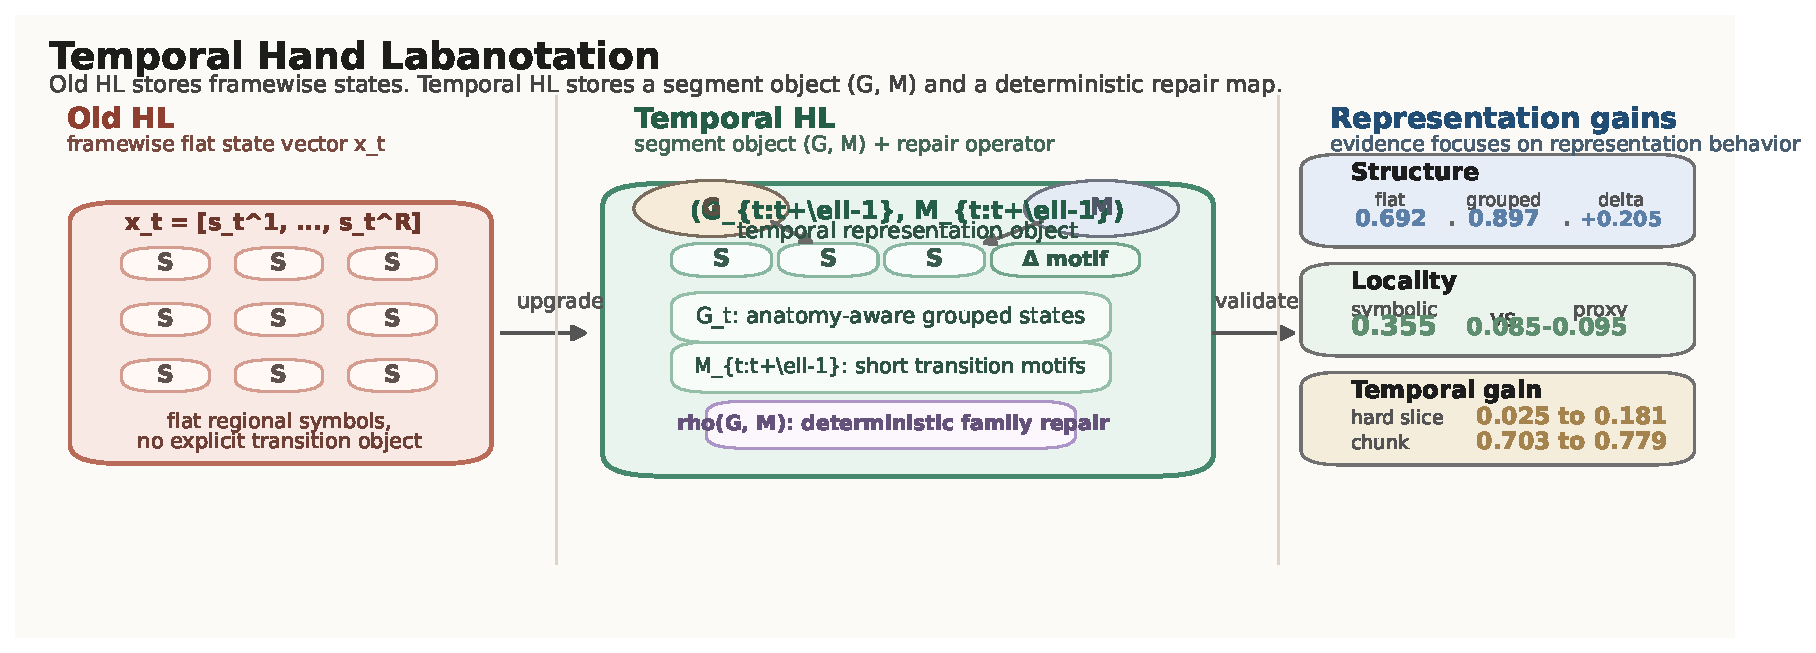
\includegraphics[width=0.96\textwidth]{Figures/temporal_hl_overview.pdf}
    \caption{Overview of \thl{}. Old HL stores each frame as a flat regional
    state vector. \thl{} stores motion with grouped symbolic states plus short
    transition motifs, then applies deterministic family repair before
    downstream use. We evaluate the resulting representation through structure,
    locality, and interaction-conditioned preservation under matched downstream
    operators.}
    \label{fig:overview}
\end{figure*}

Our contributions are:
\begin{itemize}
    \item We define \thl{}, a temporal symbolic hand-motion object that augments
    HL with anatomy-aligned grouped states, short transition motifs, and
    deterministic family repair.
    \item We show that this minimal temporal upgrade improves the properties a
    representation should expose: structure, local editability, and
    interaction-conditioned transfer.
    \item We instantiate held-out, unseen-subject evaluation protocols across
    three matched operator families so that the notation is tested as a
    representation object rather than only as the output space of a recognizer.
\end{itemize}

\section{Related Work}

\textbf{Geometric hand representations.}
Current hand representations are dominated by keypoints, meshes, and parametric
models. InterHand2.6M and FreiHAND remain standard benchmarks for 3D hand pose
and shape \citep{moon2020interhand, zimmermann2019freihand}, and MANO provides a
compact parametric hand model \citep{romero2017mano}. These representations are
effective for estimation and reconstruction, but they remain geometric objects
rather than symbolic motion units. Our goal is not to replace them for pose
recovery, but to provide a symbolic layer for motion structure that geometric
outputs do not directly expose.

\textbf{Symbolic notation for movement.}
HL introduced a symbolic vocabulary, dataset, and recognition pipeline for hand
movement documentation \citep{li2024hl}. More recent notation-driven systems
such as LabanLab emphasize that symbolic motion representations are used not
only for archival recording but also for preview, editing, and downstream
generation \citep{yan2025labanlab}. Our work builds on that notation line, but
changes the central question. Instead of translating images into per-frame
symbols more accurately, we ask what the notation object itself should contain
if it is meant to represent hand motion rather than only hand pose.

\textbf{Motion representations with temporal semantics.}
Recent motion-language work increasingly treats motion as a structured
sequence-level object rather than a stack of independent frames
\citep{chen2025language}. Large bimanual datasets and synthesis systems further
reinforce that interaction and transition structure are central to hand
behavior \citep{fu2025gigahands, zhang2025bimart}. In parallel, notation-driven
interfaces such as LabanLab show that symbolic motion objects are useful not
only for archival recording but also for preview, editing, and downstream use
\citep{yan2025labanlab}. Our setting is narrower and more symbolic: we do not
seek a foundation model for motion generation, but a compact notation-level
representation whose temporal structure is explicit, inspectable, and locally
editable. This is also the distinction from simply attaching a stronger
temporal encoder to framewise symbols: encoder-side temporalization may help
prediction, but it does not by itself yield a symbolic object that can be read,
edited, or transferred.

\section{Representation Formulation}

\subsection{Object Definition}

We formalize \thl{} as a symbolic representation for short motion segments rather
than isolated frames. Let
$x_t = (s_t^1, \dots, s_t^R)$ denote the old-HL description of frame $t$, where
each $s_t^r$ is the symbol assigned to one local hand region and $R$ is the
number of recorded regions. This frame object says what the hand state is at
time $t$, but not how nearby states are coupled over time.

\thl{} replaces this flat frame object with a temporal symbolic object
$(G_{t:t+\ell-1}, M_{t:t+\ell-1})$ over a local motion segment of length
$\ell$. The design follows three representation desiderata: anatomy-aligned
structure, explicit short-range temporal units, and symbolic consistency under
local editing and transfer. The upgrade is additive rather than destructive:
flattening the grouped state component recovers the old per-frame HL symbol
inventory, while the motif component adds the temporal information that framewise
HL does not encode. The two components serve these goals directly.

\textbf{Grouped symbolic factors.}
For each frame, the state component
$G_t = (g_t^1, \dots, g_t^F, g_t^{\mathrm{palm}})$ stores grouped symbols rather
than a flat list. The groups are anatomy-aware: the four fingers, thumb, and
hand-level structure are recorded separately so that local symbolic dependence
matches hand anatomy. The goal is not compression; it is to preserve
interpretable local independence.

\textbf{Transition chunks.}
For a contiguous run $t{:}t{+}\ell{-}1$, the motif component
$M_{t:t+\ell-1}$ stores a short symbolic transition aligned with the same
grouped states. It records how the grouped symbols evolve over the run, so
downstream retrieval and intervention operate on motion units rather than
isolated poses. Concretely, the motif is the ordered symbolic change pattern
attached to that run, not a latent hidden state used only during recognition.

\textbf{Family repair.}
Grouped states and motifs are the representation itself. We then apply a
family-level repair operator $\rho(G, M)$ that corrects residual
within-family inconsistencies while preserving symbolic intent. The operator acts
only inside anatomy-aligned families: it reconciles near-confusions among symbols
that already share the same family context, while leaving other families and the
target transition label unchanged. In this sense, $\rho(G, M)$ is a
deterministic projection back to a family-consistent symbolic object, not a
third learned component.

\subsection{Temporal Structure in the Representation}

Our design is driven by a representation question rather than a recognition
question. Simply attaching a stronger temporal encoder to framewise HL is not
the story we want to test. The representation itself must expose motion units
that exist before the encoder. We therefore organize \thl{} into three nested
levels of symbolic granularity.
\begin{itemize}
    \item \textbf{State level:} old-HL-style regional symbols remain available
    through the grouped state component $G_t$.
    \item \textbf{Grouped level:} these symbols are re-indexed into
    anatomy-aligned families rather than a single flat vector.
    \item \textbf{Chunk level:} the motif component $M_{t:t+\ell-1}$ captures
    the smallest temporal unit that still changes downstream preservation
    outcomes on the difficult interaction slices.
\end{itemize}
This hierarchy reveals where temporal headroom remains. On our
interaction-heavy slices, sequence-level routing is too coarse, while chunk- or
run-level symbolic units still retain useful signal.

\subsection{Downstream Operators}

The representation is validated through three downstream operators. They act on
the defined object $(G, M)$ rather than redefining the representation.
This choice is deliberate. If the only evaluation were framewise recognition,
then a stronger temporal encoder could improve the score even when the notation
object itself had not become more editable or more reusable. We therefore test
the representation on the operations it is supposed to support.

\textbf{Local symbolic intervention.}
Given a target field such as interaction approach or right-hand opening, we ask
whether a symbolic intervention can change only the requested field while
preserving the others. This gives a clean locality metric.

\textbf{Transfer.}
For hand-motion targets, donor frames alone are insufficient. We therefore use
donor pairs or short chunks that already realize the requested transition. This
evaluation tests whether temporal symbolic units transfer more reliably than
framewise matches.

\textbf{Interaction-conditioned preservation.}
The most difficult slices occur when a right-hand target motion must be
preserved under interacting two-hand context. Here the evaluation uses a joint score:
\[
\text{joint score} = \text{right grouped match} \times \text{left preserve}.
\]
The right hand must match the grouped target motif, and the opposite hand must
remain preserved.

\subsection{Representation Evaluation Protocol}

The downstream protocol has two stages. First, a support pool is formed from the
validation split. For easy slices this can use strict donor matching; for hard
right-hand interaction slices it requires corrected relaxed support so that the
target-hand donor and preserve-side donor can be chosen more flexibly. Second,
the selected support item is applied either as a local symbolic rewrite or as a
transition-conditioned chunk transfer. This separation matters empirically:
support relaxation accounts for the first major jump on hard slices, while
task-specific preserve-side repair and chunk transfer provide later gains. We
keep this support bank on validation rather than test data so that the final
test evaluation remains strictly held out from support construction.
Across comparisons, the downstream operator class is held fixed and only the
underlying representation changes, so improvements cannot be explained by giving
\thl{} a privileged intervention mechanism. This is the minimal fairness
condition for a representation paper: editability, preservation, and transfer
should be attributed to the notation object rather than to a stronger
downstream solver.

\section{Experimental Setup}

We reuse the HL annotation family introduced by \citet{li2024hl}, derived from
InterHand2.6M and FreiHAND \citep{moon2020interhand,zimmermann2019freihand}.
Our experiments operate on prepared temporal symbolic splits: a large train
split for symbolic pretraining, a val split for support construction and model
selection, and a test split for final evaluation. The exported benchmark contains $967/11/23$ motion sequences and
$12{,}460/2{,}739/5{,}218$ frames in train/val/test, respectively. The val and
test splits are held out at the sequence level and also introduce unseen
subjects relative to train (subject $9$ for val; subjects $10$ and $11$ for
test). We evaluate three operator families on these held-out splits and
additionally report hard right-hand interaction slices and their
feasible interaction-rich subsets, which isolate the true two-hand preservation
difficulty from frames where the opposite hand is effectively absent.

The hard slices are defined by requested right-hand motion changes under
interaction-heavy contexts. A frame is considered \emph{feasible} if the
opposite-hand content is actually present and therefore preservable. This
distinction is necessary: without it, the full-slice score is dominated by
structurally absent-opposite-hand mass and understates the quality of the
representation on the cases that matter.

We compare \thl{} against four relevant alternatives: old HL, a flat symbolic
variant without grouped temporal factors, learned-token proxies derived from
continuous frame embeddings, and learned-token proxies derived from semantic
frame embeddings. The intervention studies further compare strict support,
corrected support relaxation, feasible-subset repair, and chunk transfer under
the same held-out support protocol. Our main metrics are mean sequence accuracy,
weighted symbolic locality under controlled edits, and joint interaction
preservation on hard two-hand slices.

The learned sequence models use three seeds $\{0,1,2\}$ and report mean
sequence accuracy. The temporal symbolic learners use window size $32$, stride
$16$, hidden dimension $128$, and $20{+}20$ pretraining/finetuning epochs. The
matched learned-token controls use the stronger schedule in our benchmark:
token codebook size $64$, maximum codebook frames $100{,}000$, pretraining
window span $186$, step $96$, and $120{+}120$ epochs. Validation selects the
learned-control hyperparameters. Chunk transfer uses the best corrected
feasible-slice setting, with opening gains stable across chunk lengths $2$--$4$.
Symbolic intervention is deterministic once the split and support bank are
fixed. For the hard interaction frontier, we additionally report bootstrap
confidence intervals and paired permutation tests over evaluation frames.
All compared representations share the same split family, held-out support
protocol, and matched learned-token controls. The question is therefore not
whether a larger temporal model can solve the task, but whether the notation
itself yields better symbolic structure under matched operator strength.

\section{Results}

\begin{table*}[t]
\centering
\caption{Main results for \thl{} as a symbolic representation. All deltas are
absolute improvements under the same held-out protocol. The table follows the
claim order of the paper: better symbolic structure, cleaner local editing, and
stronger interaction-conditioned preservation and transfer. Where applicable,
the symbol inventory and downstream operator are held fixed.}
\label{tab:main_results}
\small
\setlength{\tabcolsep}{6pt}
\begin{tabular}{@{}llccc@{}}
    \toprule
    \multicolumn{5}{c}{\textbf{A. Structure and local editability}} \\
    \midrule
    Audit & Compared against & Base & Ours & Gain \\
    \midrule
    Sequence accuracy & flat HL-style symbolic sequence & 0.6923 & \textbf{0.8974} & +0.2051 \\
    Weighted locality & semantic-token proxy & 0.0945 & \textbf{0.3553} & +0.2608 \\
    Weighted locality & continuous-token proxy & 0.0848 & \textbf{0.3553} & +0.2705 \\
    \midrule
    \multicolumn{5}{c}{\textbf{B. Hard interaction-conditioned preservation}} \\
    \midrule
    Setting & Compared against & Close & Open & Gain \\
    \midrule
    Strict full slice & no support correction & 0.0250 & 0.0533 & baseline \\
    Corrected support relaxation & strict full slice & 0.1807 & 0.1812 & +0.1556, +0.1279 \\
    Feasible two-hand subset & corrected full slice & 0.6392 & 0.6497 & +0.4585, +0.4685 \\
    Preserve-side repair & feasible two-hand subset & \textbf{0.6582} & \textbf{0.6497} & +0.0190, unchanged \\
    \midrule
    \multicolumn{5}{c}{\textbf{C. Broader feasible chunk transfer}} \\
    \midrule
    Operator & Compared against & Close & Open & Gain \\
    \midrule
    Fixed-edge transfer baseline & single donor edge match & 0.7025 & 0.6306 & baseline \\
    Chunk transfer & fixed-edge transfer baseline & \textbf{0.7785} & \textbf{0.7197} & +0.0760, +0.0891 \\
    \bottomrule
\end{tabular}
\end{table*}

\subsection{Main Results}

Table~\ref{tab:main_results} gives the paper's central verdict. Across all three
blocks, \thl{} is stronger precisely where the evaluation depends on explicit
symbolic structure rather than on framewise matching alone.
Table~\ref{tab:ablation}, the paper's only ablation table, then isolates which
temporal channels are responsible for those gains.
Taken together, these tests answer the representation question directly:
structure tests ask whether the notation organizes state better, locality tests
ask whether edits stay local, and interaction-preservation tests ask whether the
same object can preserve motion under downstream use.
Where applicable, the symbol inventory, operator class, and support protocol
are held fixed, so the gains are evidence about the representation rather than
about a privileged solver. The same pattern holds on unseen-subject held-out
splits rather than only on in-distribution motion fragments.

\subsection{Structure and Locality}

The first block establishes the representation claim directly. Grouping the
state factors raises sequence accuracy from $0.6923$ to $0.8974$, a gain of
$+0.2051$ without changing the symbol inventory, so the improvement comes from
how the notation organizes motion state rather than from enlarging the
vocabulary. The same block shows a large locality margin: weighted symbolic
locality reaches $0.3553$, while matched semantic and continuous learned-token
proxies remain at $0.0945$ and $0.0848$. When an edit must change one field
while preserving the rest, the symbolic structure isolates the requested change
far better than proxy token spaces trained only for generic separability.

\subsection{Hard Interaction Preservation}

The hardest setting is right-hand motion preservation under interaction, and it
is also where frame-only HL is least adequate. Corrected support relaxation
already raises joint success to $0.1807$ for closing and $0.1812$ for opening.
Once evaluation is restricted to genuinely feasible two-hand cases, the same
representation reaches $0.6392$/$0.6497$, and preserve-side repair further
lifts closing to $0.6582$ while maintaining $0.6497$ on opening. The gain only
appears once target motion and opposite-hand preservation are evaluated
together rather than matched independently.

These gains are statistically stable. On the full hard slice, corrected support
relaxation improves closing by $+0.156$ (95\% CI $[0.127, 0.186]$) and opening
by $+0.128$ (CI $[0.101, 0.156]$), with paired permutation tests below
$10^{-4}$ in both cases. On the feasible interaction subset, preserve-side
repair adds another $+0.184$ on closing ($[0.108, 0.259]$, $p = 5\times10^{-5}$)
and $+0.166$ on opening ($[0.108, 0.223]$, $p < 10^{-4}$).

These results show that temporal symbolic quality becomes visible only once the
evaluation respects the two-hand constraint. After target matching is handled
correctly, the remaining headroom lies in preserve-side consistency, so the
later gains come from repair and chunk transfer rather than donor selection
alone.

\subsection{Chunk-Level Transfer}

Chunk transfer gives the clearest temporal gain on broader corrected feasible
slices: Table~\ref{tab:main_results} shows improvements from $0.7025$ to
$0.7785$ on closing and from $0.6306$ to $0.7197$ on opening. The opening gain
is stable across chunk lengths $2$, $3$, and $4$, which indicates that the
benefit comes from short local transition structure rather than long-horizon
modeling. Table~\ref{tab:ablation} aligns with this result within the learned
sequence-model family: the best formulation is symbolic state plus short
transition channels, while heavier duration and coordination channels do not
match it and the learned-token control remains well below it. The paired slice
comparison is also clean: on
broader feasible closing, chunk transfer wins on $12$ frames, loses on $0$, and
ties on $146$; on opening, it wins on $14$, loses on $0$, and ties on $143$.

\begin{center}
\captionsetup{type=table}
\captionof{table}{Representation ablation within the learned sequence-model
family. The best formulation is the minimal temporal upgrade: symbolic state
plus short transition motifs. Deltas are reported against the best row.}
\label{tab:ablation}
\small
\begin{tabular}{@{}p{0.56\columnwidth}cc@{}}
    \toprule
    Formulation & Seq. acc. & $\Delta$ vs best \\
    \midrule
    State + transition & \textbf{0.9231} & best \\
    State + transition + duration & 0.8205 & -0.1026 \\
    State only & 0.7949 & -0.1282 \\
    State + transition + coordination & 0.7436 & -0.1795 \\
    Learned-token control (64) & 0.6923 & -0.2308 \\
    \bottomrule
\end{tabular}
\end{center}

\subsection{Temporal Granularity Analysis}

The remaining gap localizes where stronger symbolic supervision is still needed.
Interaction preservation improves sharply once support is corrected and
evaluation focuses on feasible two-hand cases, while chunk transfer adds a
second gain layer on broader feasible slices. The residual difficulty is now
concentrated on preserve-side consistency in interaction-heavy cases, not on
whether temporal structure belongs in the representation.

\section{Discussion and Limitations}

\thl{} upgrades HL into a hand-motion representation with explicit short-range
temporal structure. Relative to frame-only HL, it better preserves structure,
supports local edits, and transfers motion under interaction. The strongest
gains appear exactly where the evaluation depends on temporal symbolic content.

The upgrade is also minimal in the right way. \thl{} preserves the original HL
inventory, reorganizes it into anatomy-aligned state factors, and adds short
transition motifs only where framewise notation is insufficient. This keeps the
notation compatible with HL while changing what downstream symbolic operators
can do.

This is also why we emphasize representation-level evidence rather than
recognition-only gains. For a notation paper, the strongest claim is not that a
decoder can classify frames more accurately, but that the symbolic object
supports the operations for which a notation is actually used.

We also keep the scope of that claim narrow. The paper does not argue that
these tests exhaust every downstream use of hand notation; it argues that they
cover the core operations a symbolic hand-motion representation should support
before broader generalization is considered.

The current frontier is preserve-side consistency under dense interaction. The
remaining headroom lies at run or chunk granularity, where simple symbolic
selectors do not yet recover all feasible context. A natural next step is
interaction-aware temporal supervision. We keep the present study within the
HL-derived benchmark so that the gains reported here remain attributable to the
representation itself.

\section{Conclusion}

\thl{} is a symbolic representation for hand motion with short transition
structure inside the notation. Relative to a frame-only formulation, it
preserves structure more reliably, supports local editing, and improves motion
transfer under interaction. Time-local transition structure belongs to the
representation itself, not to an optional decoder-side refinement. The
resulting notation object supports retrieval, intervention, reuse, and more
direct symbolic interfaces for downstream hand-motion systems.

\bibliography{references}

\end{document}
